\chapter{Analyse af problemområdet}
\label{chap:analyseafpo}

I følgendende kapitel vil vi analysere problemområdet. Analysemetoden tager udgangspunkt metoden beskrevet i bogen Objektorienteret Analyse \& Design (OOA\&D)\cite[s. ~43]{ooad}. Problemområdet er den del af omgivelserne, som skal administreres, styres og overvåges af vores system, Foodl. I vores tilfælde er problemområdet: madresterne og madlavningen i de danske hustande. Formålet med analysen, er at skabe et overblik over, hvilke klasser og hændelser Foodl skal have, for at kunne udføre de funktioner vi ønsker, og for at systemet bliver så brugbart som muligt for dets fremtidige brugere. 



% Problemområde
\section{Klasser}
\label{sec:klasser}
Vi ønsker nu at vælge de bestanddele, som vi vil modellere i problemområdet. Disse vælges
ved at kigge på systemdefinitionen og ved at fremstille rige billeder (se \todo{bilag}).

Grundet den iterative arbejdsproces, er klasser undervejs blevet tilføjet og fjerent, og vi ønsker nu at kaste lys over baggrunden bag de valgte klasser. I gennem processen har vi også fravalgt klasser. Disse, med beskrivelse, kan findes i \apref{ap:fravalgteklasser}.

\subsection{Valgte klasser}
Herunder ses de valgte klasser og hvorfor vi vælger at have dem med i vores model af problemområdet.
Vi mener at disse klasser samler de objekter og hændelser, som er relevant for denne model af problemområdet.

\begin{description}
\item[Ingrediens] \hfill \\ 
I opskrifter bruges der flere ingredienser. En ingrediens består af en råvare og en mængde af denne. Det er et problem at finde opskrifter, der indeholder ingredienser svarende til de råvarer man har til rådig. Det er et problem for informanterne at maden laves i for store portioner, altså er det et problem hvis en opskrifts ingredienser indeholder store mængder.

\item[Bogmærke] \hfill \\
Det er en del af problemområdet, for brugere at huske de gode opskrifter. Der vil til tider blive benyttet en opskrift, der er så god, at den er værd at gemme til en anden gang. Derfor beholder vi denne klasse.

\item[Råvare] \hfill \\
En råvare findes i køleskabene og på madhylderne i husholdningerne. Det er et problem at finde opskrifter, der kun indeholder disse råvarer, derfor skelnes der mellem ingredieser og råvarer.

\item[Indkøbsliste] \hfill \\
Vi vurderer, at der i en husholdning ofte bliver skrevet en indkøbsliste med de ting man mangler. Indkøbslisten kan være skrevet på baggrund af en opskrift man gerne vil lave, eller en hel madplan man gerne vil følge over en længere periode.

\item[Opskrift] \hfill \\
En opskrift er det centrale i problemområdet. Opskrifterne indeholder forskellige ingredienser. Det er nødvendigt at have råvarer nok til at matche ingredienserne i opskriften, før denne kan laves. Man må gå ud fra at den typiske private madlaver har mange opskrifter i kogebogen, som han/hun reelt ikke har råvarerne til at kunne lave.
\end{description}

\subsection{Struktur}

De valgte klasser giver anledning til et klassediagram. Dette kan ses i \figref{fig:klassediagram}. 

\begin{figure}
  \centering
  \input{billeder/klassediagrampo.pdf_tex}
  \capt{Klassediagram for problemområdet.}
  \label{fig:klassediagram}
\end{figure}


Klassediagrammet ovenover er bygget op af aggregeringer og associationer imellem klasserne i diagrammet. For konkrete beskrivelser af de forskellige klasser, konsulteres hændelses- og klassebeskrivelserne. Her beskrives relationen mellem klasserne.

\begin{description}
  \item[Bogmærke] \hfill \\
    En bogmærke kan repræsentere opskrifter.

  \item[Opskrift] \hfill \\
    Består udelukkende af ingredienser og har fremgangsmåden som attribut. En opskrift kan bogmærkes en gang pr. bruger. Som minimum består en opskrift af en ingrediens.
Attributter: Titel, Billede, Fremgangsmåde

\item[Indkøbsliste] \hfill \\
  Indkøbslisten består udelukkende af en til flere ingredienser, der tilføjes ud fra opskrifterne. Derudover er det muligt at yderligere tilføje elementer på indkøbslisten i form af arbitrære tekststrenge.

\item[Ingrediens] \hfill \\
  En ingrediens består af en råvare.
Attributter: Mængde, Enhed

\item[Råvare] \hfill \\
  En råvare er en dekomponering af en ingrediens. En råvare er blot en ingrediens uden nogen form for information om mængde eller enhed. En ingrediens kunne for eksempel være 200g oksekød.
Attributter: Navn
\end{description}

 
\section{Struktur}
\label{sec:struktur}

Sturkturen på vores klasser beskrives ved hjælp af et klassediagram. Med et klassediagram, skabes der et overblik over relationen mellem de forskellige klasser og objekter. \Foodl{} består af 6 klasser, nemlig ``Opskrift'', ``Vare'', ``Råvare'', ``Ingrediens'', ``Fejl'' og ``Person''. Relationen mellem klasserne kan ses i klassediagrammet i \figref{fig:klassediagram}. En relation mellem to klasser markeret med en rumbe-pil, er en aggregerings-struktur, hvilket er en relation som beskrives ved udsagnet ``har-en'' og ``indgår-i''. Eksempelvis, så er råvare en aggregering af ingrediens, hvilket betyder at en ingrediens ``har-en'' råvare, og en råvare ``ingår-i'' og er en dekomponering af en ingrediens. Dette indgår samtidig i et hierarkimønster, idet opskrifter aggregerer ingredienser, som aggregerer en råvare. En relation mellem to klasser markeret med en streg, er en associeringsstruktur, som betyder at de to klasser har en sammenhæng. I vores struktur, associerer klasserne fejl og opskrifter med hinanden. En associering er ikke, ligesom en aggregering, nem at knytte et udsagn til. Men i vores tilfælde kan en associering mellem fejl og opskrift beskrives som et ``hører-til''-forhold. Fejl ``hører-til'' en opskrift, og en opskrift kan muligvis ``høre-til'' fejl. Hver relation har desuden multipliciteter tilknyttet. Dette beskriver forholdet mellem klasserne. Det kan eksempelvis være et et-til-et-forhold, eller et 0-til-mange-forhold. På \figref{fig:klassediagram} ses det, at forholdet mellem klassen opskrift, og klassen ingrediens er et 1-til-mange-forhold (*-tegnet betyder mange), mens forholdet mellem ingrediens og opskrift er et 1-forhold. Det betyder altså at der på hver opskrift er minimum én ingrediens, og at hver ingrediens hører til præcis én opskrift. Hver enkelt klasses relationer, forhold og multiplicitet, forklares herunder nærmere:

\begin{figure}
  \centering
  \input{billeder/klassediagrampo.pdf_tex}
  \capt{Klassediagram for problemområdet.}
  \label{fig:klassediagram}
\end{figure}



\begin{description}

\item[Associering mellem person og vare (indkøbsliste)] \hfill \\
En person associerer 1-til-mange varer, modelleret på baggrund af indkøbslisten. En indkøbsliste kan benyttes af en person til at holde styr på hvilke varer, der skal handles ind.  Det er muligt for en person være relateret til mange vare. Hvert vareobjekt er unikt for hvert personobjekt, dvs. at det altså ikke muligt for personer, at dele varer mellem sig. En indkøbsliste kunne have været en klasse for sig selv, men fordi hver person kun har netop en indkøbsliste, er dette overflødigt.

\item[Associering mellem person og fejl] \hfill \\
Fejl associerer med bruger-klassen, da det er brugeren, der opdager fejl. En bruger kan opdage flere fejl i den samme, eller forskellige opskrifter i løbet af brugerobjektets levetid.

\item[Associering mellem opskrift og fejl] \hfill \\
En opskrift kan bestå af 0-til-mange fejl. Hvis opskriften er dårligt fremstillet eller kommer fra en hjemmeside, hvor brugere selv kan tilføje og dele opskrifter, kan der \fx være mange fejl i en enkelt opskrift. Hvis opskriften derimod stammer fra en kilde med revidering før udgivelse, \fx en opskriftsamling eller Arlas Karolines Køkken, vil der højst sandsynligt ikke være nogle fejl. 

\item[Associering mellem opskrift og person (bogmærke)] \hfill \\
Personer kan associeres med flere opskrifter i et forhold udtrykt som bogmærker. Støder personen på en opskrift, som personen synes er god, og ønsker at gøre den let tilgængelig til en anden gang, så skal det være muligt at bogmærke denne. Et bogmærke er dog ikke udtrykt i modellen som en klasse, da hvert bogmærke ikke har nogen identitet, udover associeringen med en opskrift og en person. Hver opskrift kan derudover også associeres med flere personer, dvs. at flere forskellige personer godt kan have et bogmærke på den samme opskrift. 

\item[Aggregering mellem opskrift og ingrediens] \hfill \\
En opskrift består af 1-til-mange ingredienser. Hvis opskriften ikke bestod af nogle ingredienser, ville det ikke være en opskrift og skulle derfor ikke modelleres. Hver ingrediens tilhører netop en opskrift.

\item[Aggregering mellem ingrediens og råvare] \hfill \\
Hver opskrift består af netop en råvare, mens en råvare kan tilhøre mange forskellige ingredienser. Ingrediensen ``300 g hvedemel'' består \fx af råvaren ``Hvedemel''.

\end{description}

            
\section{Adfærd}
\label{sec:adfaerd}

De forskellige klasser og hændelser i problemområdet er nu blevet analyseret og beskrevet. Alle hændelsesforløb, der er mulige for alle objekter i en klasse, kan beskrives ved hjælp af adfærdsmønstre\cite[s.~90]{ooad}. Den objektorienterede tilgang er baseret på, at der i vores systems model skal være et objekt for hvert objekt i problemområdet\cite[s.~91]{ooad}. Hvert objekt skal registrere og huske adfærden af det tilsvarende objekt i problemområdet, som det ændrer sig over tid.

For hver klasse følger er der en tilhørende figur, som illusterer klassens adfærd. I figurene er der et start  der bokse og pile. De afrundede rektangulære bokse med tekst, skal anses som tilstande, som den pågældende klasse kan have. Pilene der fører til en tilstand, skal anses som hændelser, som kan være skyld i et tilstandsskift.

\subsection{Indkøbsliste}
\label{subsec:brug-indkoebsliste}

Ud over muligheden for at tilføje opskrifternes ingredienser til indkøbslisten, så kan man også tilføje almindelig tekst til, så det er muligt at lave en indkøbsliste, der indeholder andet end ingredienser til madlavningen. Så man kan skrive andre varer på, som man kan købe med fra \fx supermarkedet. Systemets indkøbsliste kan ses i \figref{fig:overblik-indkoebsliste}.

\begin{figure}[H]
	\centering
	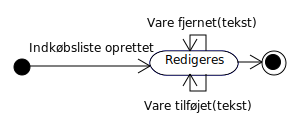
\includegraphics[scale=1]{billeder/foodl/thumbnails/indkoebsliste.png}
	\capt{Denne figur har til formål at give et overblik over systemets indkøbsliste.}
	\label{fig:overblik-indkoebsliste}
\end{figure}

Brugeren har mulighed for at tilføje varer i feltet ``tilføj til indkøbsliste'' og trykke på ``tilføj'' i bunden af siden. Der er mulighed for at slette alle varer fra indkøbslisten, ved at trykke på knappen ``slet alt'' i øverste højre hjørne af indkøbslisten, og ligeledes at slette enkelte varer, ved at trykke på de små gule krydser ud for alle varerne. Derudover er der implementeret en knap, til at udskrive indkøbslisten, som vi naturligvis kalder for ``udskriv''.

Hvis brugeren ikke er logget ind, vil de se i øverste højre hjørne af \figref{fig:overblik-indkoebsliste} (under sidehovedet) en boks, som informerer brugeren om, at man skal være logget ind for at systemet skal være i stand til at gemme indkøbslisten og favoritter. Oprettelse af bruger og indlogning bliver beskrevet nærmere i \secref{subsec:brug-opret}.

\subsection{Råvare}
Når nogen i sin husstand køber en råvare, indtræffer hændelsen \textit{råvare købt}. Denne hændelse fører råvare-klassen i en ny tilstand, der hedder \textit{brugbar}. Denne råvare er klar til at blive brugt. Inden der bliver handlet ind, og inden der sker et tilstandsskift, så er råvaren i en tidligere tilstand, der hedder \textit{eksisterer}. Dette tilstandsdiagram har ikke en afsluttendde hændelse, fordi vi har vurderet, at en råvare altid vil eksistere. Men den er først brugbar, når man har købt den. 

Indehaverne af en råvare har nu to muligheder. Man kan enten bruge hele råvaren, eller man ende med at smide noget af den ud. Disse to hændelser har vi samlet under en fælles hændelse, som vi kalder \textit{råvare opbrugt}. Denne hændelse fører klassen i en gammel tilstand, der hedder \textit{eksisterer}, da den ikke længere er brugbar i husstanden. Se \figref{fig:raavare-adfaerd}.

\begin{figure}[H]
	\centering
	\scalebox{0.8}{
	\subsection{Råvare}
Når nogen i sin husstand køber en råvare, indtræffer hændelsen \textit{råvare købt}. Denne hændelse fører råvare-klassen i en ny tilstand, der hedder \textit{brugbar}. Denne råvare er klar til at blive brugt. Inden der bliver handlet ind, og inden der sker et tilstandsskift, så er råvaren i en tidligere tilstand, der hedder \textit{eksisterer}. Dette tilstandsdiagram har ikke en afsluttendde hændelse, fordi vi har vurderet, at en råvare altid vil eksistere. Men den er først brugbar, når man har købt den. 

Indehaverne af en råvare har nu to muligheder. Man kan enten bruge hele råvaren, eller man ende med at smide noget af den ud. Disse to hændelser har vi samlet under en fælles hændelse, som vi kalder \textit{råvare opbrugt}. Denne hændelse fører klassen i en gammel tilstand, der hedder \textit{eksisterer}, da den ikke længere er brugbar i husstanden. Se \figref{fig:raavare-adfaerd}.

\begin{figure}[H]
	\centering
	\scalebox{0.8}{
	\input{billeder/tilstandsdiagrammer/raavare.pdf_tex}}
	\capt{Tilstandsdiagram for klassen råvare. De afrundede rektangulære bokse med tekst, skal anses som tilstande, som klassen kan have. De pile, der fører til en tilstand, skal anses som hændelser, som kan være skyld i et tilstandsskift. I dette tilfælde har klassen to tilstande (eksisterer) og (brugbar). Dette tilstandsdiagram har ikke en afsluttendde hændelse.}
	\label{fig:raavare-adfaerd}
\end{figure}}
	\capt{Tilstandsdiagram for klassen råvare. De afrundede rektangulære bokse med tekst, skal anses som tilstande, som klassen kan have. De pile, der fører til en tilstand, skal anses som hændelser, som kan være skyld i et tilstandsskift. I dette tilfælde har klassen to tilstande (eksisterer) og (brugbar). Dette tilstandsdiagram har ikke en afsluttendde hændelse.}
	\label{fig:raavare-adfaerd}
\end{figure}
\subsection{Opskrift}
En opskrift kan befinde sig i en kogebog, på et stykke papir eller på en hjemmesiden. I \figref{fig:opskrift-adfaerd}, ses adfærden for klassen ``Opskrift''. En opskrift kommer til live, ved hændelsen \textit{opskrift fundet}. Her befinder den sig i tilstanden \textit{findes i opskriftssamlingen}. Hvis man er rigtig glad for en opskrift, kan man sætte et bogmærke på opskriften, så man hurtigt kan finde den igen. Sådan en hændelse kaldes for \textit{bogmærke tilføjet}. Hvis man ombestemmer sig og fjerner bogmærket, indtræffer hændelsen \textit{bogmærke fjernet}. Derudover kan man være nødsaget til at handle ind til en specifik opskrift, fordi man mangler nogle ingredienser. Det betyder, at man skal tilføje nogle opskrifter til en indkøbsliste. Denne hændelser kaldes for \textit{skrevet på indkøbsliste} med den modsignende hændelse \textit{fjernet fra indkøbsliste}. Der kan også eksistere en fejl i opskriften. En fejl kunne være et manglende billede til opskriften, eller at der står 20 minutter i ovnen i stedet for 40. Dette er beskrevet ved hjælp af hændelsen ``fejl fundet''. Disse fire hændelser medfører ikke et tilstandsskift. Opskriften ryger kun ud af tilstanden \textit{findes i opskriftssamlingen}, når opskriften fjernes, vha. hændelsen \textit{opskrift smidt ud}..

\pdffig[0.8]{tilstandsdiagrammer/opskrift}
  {Tilstandsdiagram for klassen opskrift. Klassen har én tilstand (findes i opskriftssamlingen) og en afsluttende hændelse ``opskrift fjernet'', der fører klassen ud i en sluttilstand.}
  {fig:opskrift-adfaerd}

\subsection{Bogmærke}
Som nævnt kan man vælge at tilføje et bogmærke til en opskrift, man kan lide. Denne hændelse kaldes \textit{bogmærke sat ind}, og bringer klassen i tilstanden \textit{aktiv}. Bogmærket er aktiv, indtil den kommer i sluttilstanden efter, at hændelsen \textit{bogmærke fjernet} indtræffer. Se \figref{fig:bogmaerke-adfaerd} for tilstandsdiagrammet over denne klasse.

\pdffig[0.8]{tilstandsdiagrammer/bogmaerke}
  {Tilstandsdiagram for klassen bogmærke. Klassen har én tilstand (aktiv) og en afsluttende hændelse ``bogmærke fjernet'', der fører klassen ud i sluttilstanden.}
  {fig:bogmaerke-adfaerd}

\subsection{Ingrediens}

\todo{Revider hele dette afsnit!}
En ingrediens kommer til verdenen sammen med en opskrift. Dette er fordi, at en ingrediens ikke er en del af problemområdet før den optræder i en opskrift. Det er nemlig først der, at man i en husstand behøver at bekymre sig om ingredienser. Hvis de ikke fandtes i nogle opskrifter, var der ikke nogen grund til at indkøbe en råvare svarende til ingrediensen, og ingrediensen ville derved ikke være en del af problemområdet. Denne hændelse kaldes \textit{Opskrift fundet}. Mens ingrediensen ekisister, er den i tilstanden af samme navn. Når man kender til en ingrediens, kan man skrive den på sin indkøbsliste. Dette gør man hvis man vil være sikre på at huske at købe en råvare svarende til ingrediensen, når man er ude at handle ind. Man kan selvfølgelig også fjerne ingrediensen fra sin indkøbsliste, hvis man har ombestemt sig og ikke ønsker at huskes på at købe den tilsvarende råvare. Disse to hændelser kaldes \textit{ingrediens tilføjet} og \textit{ingrediens fjernet}. Når opskriften, der indeholder en given ingrediens, smides ud, er hændelsen \textit{Opskrift smidt ud} netop indtruffet, og ingrediensen bringes i sin sluttilstand. Det bør bemærkes, at 2 forskellige opskrifter, der begge indeholder pasta, anses for at indeholde hver sin ingrediens. Dette er en vigtig adskillelse, da ingredienser består af en mængde og enhed, \fx 200 g pasta.

\begin{figure}[H]
	\centering
	\scalebox{0.6}{
	\subsection{Ingrediens}

\todo{Revider hele dette afsnit!}
En ingrediens kommer til verdenen sammen med en opskrift. Dette er fordi, at en ingrediens ikke er en del af problemområdet før den optræder i en opskrift. Det er nemlig først der, at man i en husstand behøver at bekymre sig om ingredienser. Hvis de ikke fandtes i nogle opskrifter, var der ikke nogen grund til at indkøbe en råvare svarende til ingrediensen, og ingrediensen ville derved ikke være en del af problemområdet. Denne hændelse kaldes \textit{Opskrift fundet}. Mens ingrediensen ekisister, er den i tilstanden af samme navn. Når man kender til en ingrediens, kan man skrive den på sin indkøbsliste. Dette gør man hvis man vil være sikre på at huske at købe en råvare svarende til ingrediensen, når man er ude at handle ind. Man kan selvfølgelig også fjerne ingrediensen fra sin indkøbsliste, hvis man har ombestemt sig og ikke ønsker at huskes på at købe den tilsvarende råvare. Disse to hændelser kaldes \textit{ingrediens tilføjet} og \textit{ingrediens fjernet}. Når opskriften, der indeholder en given ingrediens, smides ud, er hændelsen \textit{Opskrift smidt ud} netop indtruffet, og ingrediensen bringes i sin sluttilstand. Det bør bemærkes, at 2 forskellige opskrifter, der begge indeholder pasta, anses for at indeholde hver sin ingrediens. Dette er en vigtig adskillelse, da ingredienser består af en mængde og enhed, \fx 200 g pasta.

\begin{figure}[H]
	\centering
	\scalebox{0.6}{
	\input{billeder/tilstandsdiagrammer/ingrediens.pdf_tex}}
	\capt{Tilstandsdiagram for klassen ingrediens. I dette tilfælde har klassen én tilstand, nemlig eksisterer, og en afsluttende hændelse, der fører klassen ud i en sluttilstand.}
	\label{fig:ingrediens-adfaerd}
\end{figure}}
	\capt{Tilstandsdiagram for klassen ingrediens. I dette tilfælde har klassen én tilstand, nemlig eksisterer, og en afsluttende hændelse, der fører klassen ud i en sluttilstand.}
	\label{fig:ingrediens-adfaerd}
\end{figure}

        

